\section{Standing Up the Z80}

Let's start this process by making sure we can get our Z80 processor to work properly. Building incrementally, and learning as we go,
is key to how we are approaching the creation of our Retro Computer. Following a similar approach will be helpful for you as you explore new components and systems of your own design.

We want to minimize the number of failure points, so we are going to take our first steps with the Z80 using the Arduino as our bootstrap. We know we are working with a +5V processor expecting TTL-level logic signals, so the Arduino will interface without having to do any special level shifting. What we need to do is to ascertain the \textit{bare minimum} we need to do to the Z80 to make it function (and, of course, we need some way of confirming that the processor \textit{is} doing something!).

What's the simplest thing we can have the Z80 do? Without any memory, we can't provide the Z80 with any kind of interesting program to run. Without any I/O devices, we can't enter data or see the results of any program anyway. Instead, we will \textit{trick} the Z80 into thinking it is reading a program from memory - but it will be the world's most boring program, and endless series of NOP instructions.

NOP stands for \textit{no operation}. It's an instruction that effectively does nothing, other than to tell the processor to move on to the next instruction. An endless series of of NOPs will cause the processor to run forever, doing 'nothing' but looking at memory address after memory address, finding NOP after NOP. What helps us out here is that the binary code for NOP is 00000000.

We don't have to build any kind of memory into this exiprement; we simply need to ensure that whenever the Z80 tries to read from memory looking for an instruction, that all of the data lines are 0. It will think it has read from memory and found a NOP.

Since the Z80 will execute the NOP then move to the next address, we can check to see if the Z80 is working by looking at the address bus. If we connect some LED's to the bus, we should see them turn on and off in an ascending binary pattern every few clock ticks (it takes the Z80 multiple clock ticks to execute an instruction).

Reviewing the datasheet, we see have a number of pins on the Z80 that we will need to do something with:

\resizebox{\textwidth}{!}{%
\begin{tabular}{|c|c|l|}
\hline
\textbf{Pin} & \textbf{Name} & \textbf{Notes} \\
\hline
$A_{0}$ - $A_{15}$ & Address Bus & We will use the address bus to view the actions of the processor. \\
\hline
$D_{0}$ - $D_{7}$ & Data Bus & We need to tie these low to simulate a NOP instruction. \\
\hline
$M_{1}$ & Machine Cycle One & This is an output pin, which we can ignore. \\
\hline
$MREQ$ & Memory Request & This is an output pin, which we can ignore. \\
\hline
$IORQ$ & Input/Output Request & This is an output pin, which we can ignore. \\
\hline
$RD$ & Memory Read & This is an output pin, which we can ignore. \\
\hline
$WR$ & Memory Write & This is an output pin, which we can ignore. \\
\hline 
$REFSH$ & Refresh & This is an output pin, which we can ignore. \\
\hline
$HALT$ & Halt & This is an output pin, which we can ignore. \\
\hline
$WAIT$ & Wait & We need to turn this pin off or the Z80 will enter into a waiting state. \\
\hline
$INT$ & Interrupt Request & We need to turn this input pin off. \\
\hline
$NMI$ & Non-Maskable Interrupt & This also needs to be turned off. \\
\hline
$RESET$ & Reset & We will need to temporarily activate this pin to get the Z80 started properly. \\
\hline
$BUSRQ$ & Bus Request & Another input pin that needs to be turned off. \\
\hline
$BUSAK$ & Bus Acknowledge & This is an ouput pin, which we can ignore. \\
\hline
$CLK$ & Clock & We need to provide a clock signal to the Z80. \\
\hline
\end{tabular}}

\begin{center}
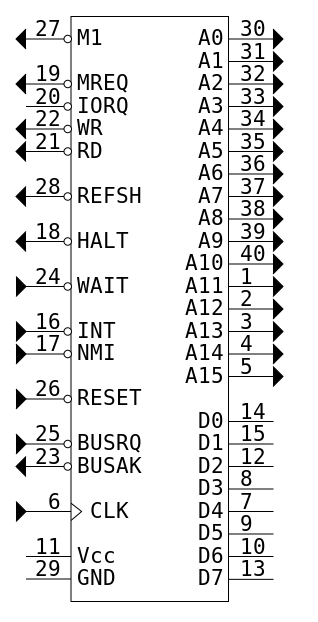
\includegraphics[height=6cm]{Z80_pinout.png}
\end{center}

Some comments:

\begin{itemize}
\item The WAIT, INT, NMI and BUSRQ pins are \textbf{active low}. This means that the pin's logic levels are effectively inverted; a 'low' is ON or 1, a 'high' is OFF or 0. To turn these pins off, we must actually provide +5V. 
\item The Data Bus is not inverted; it is \textbf{active high}. With any IC, though, we can't leave an input pin unconnected and just assume that it will be a zero (the Data Bus are tri-state, input/output pins). We need to explicitly set it low, which we do by connecting the pin to ground through a small resistor.
\end{itemize}

It looks like there are a number of pins we can either safely ignore, or simply tie to either +5V or ground. And although we didn't list them, we do need to provide +5V of power and make a ground connection. 

\subsection{Schematic}
\begin{center}
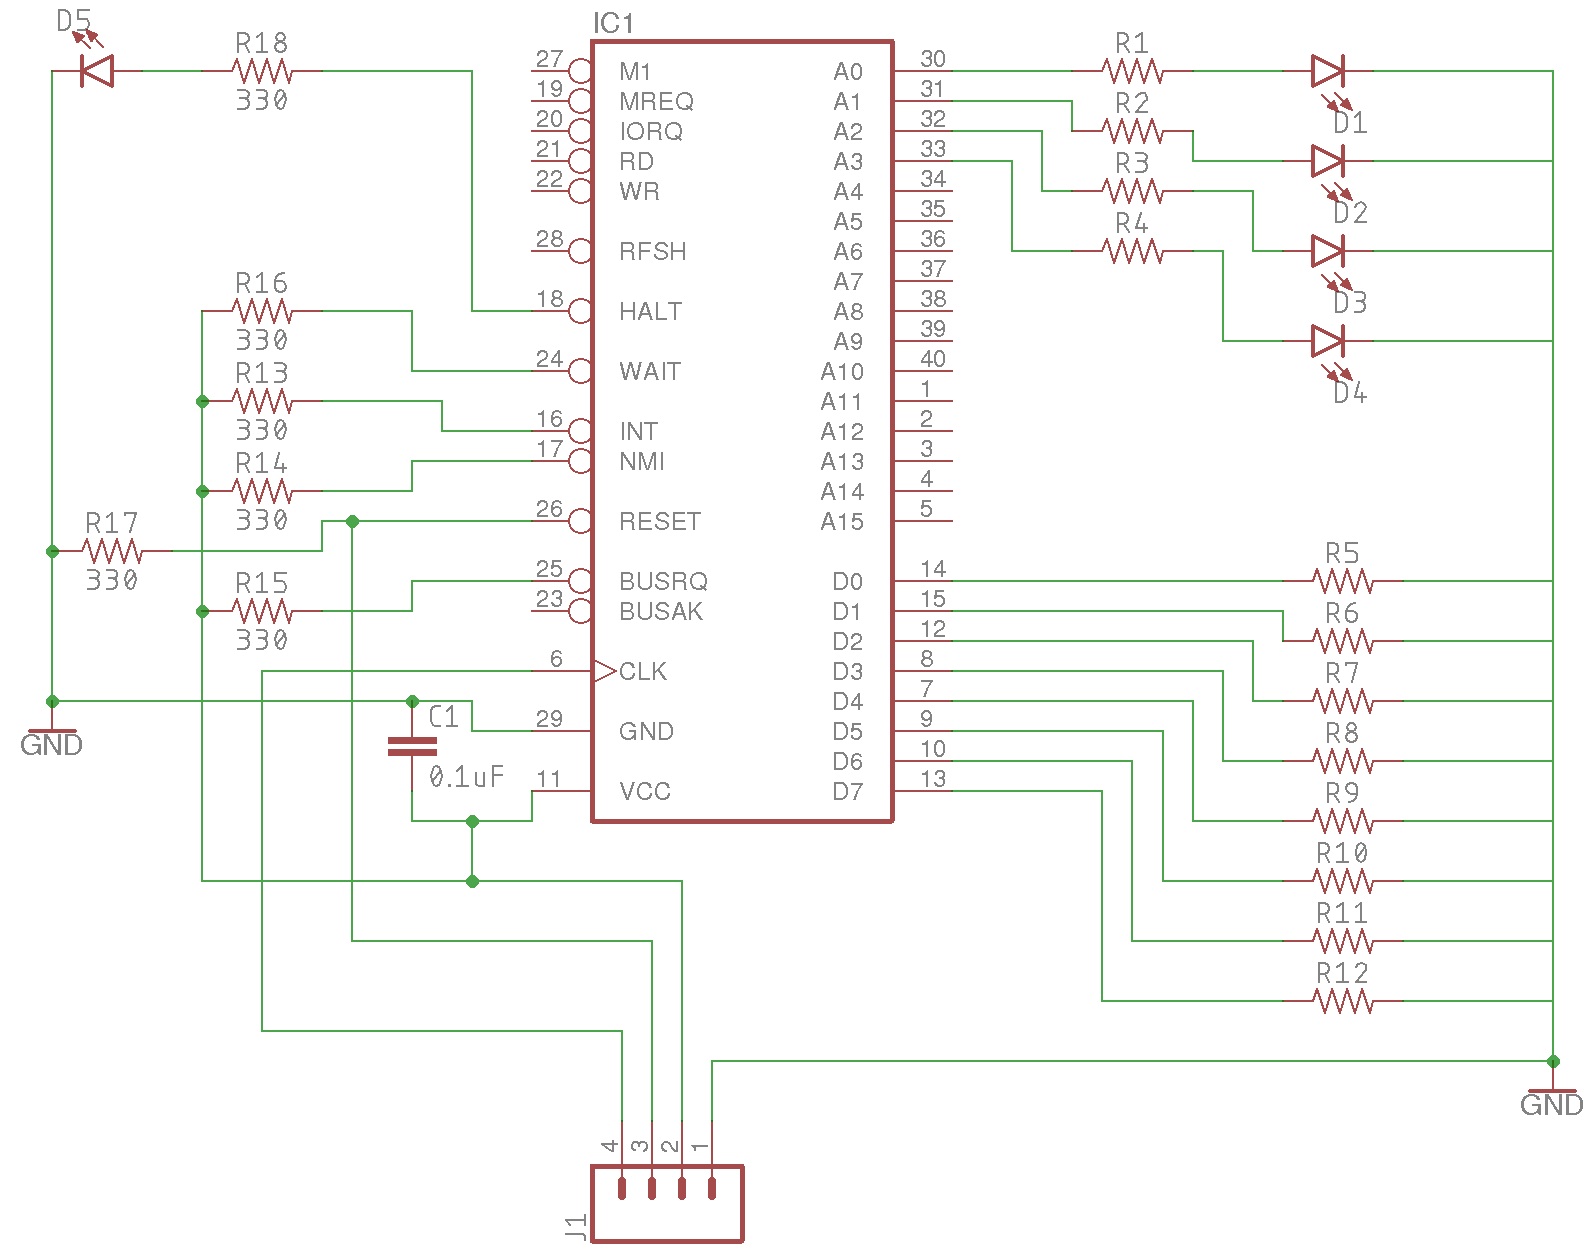
\includegraphics[height=10cm]{first_z80_schematic.png}
\end{center}

Let's walk through the schematic connection by connection:

\begin{itemize}
\item Address lines $A_{0}$ through $A_{3}$ are connected to a resistor then to an LED. These pins will provide $+5V$ when on, so we need to be sure we connect to the proper side of the LED (the longer wire on an LED is positive). The other side of the LED goes into ground\footnote{The resistor can vary depending on the LED, but assuming you are using a standard red LED, a resistor of around 220 ohms should be fine. The purpose of the resistor is to drop some of the voltage, as putting $+5V$ directly on the LED can and probably will burn it out, imediatly if not eventually.}.
\item We need to simulate a zero on each data line, so we tie each line to ground. We can't leave the line open; it will float around and may or may not end up as a low or zero. We could just tie it directly to ground, but we insert a 330 ohm resistor to limit the amount of current that the Z80 has to try and provide. So - data lines $D_{0}$ through $D_{7}$ each go to a resistor then to ground.
\item $WAIT$, $INT$, $NMI$, and $BUSRQ$ All need to be turned off. They are active \textbf{low}, so we need to provide a logic level high to turn them off. They are all connected through a resistor to the $+5V$ supply\footnote{In this case, the resistor is not really necessary annd if fact will drop the voltage a little but I left it in to be consistent with what I really did while building this.}.
\item In order to help debug, I added a LED to the $HALT$ line. This is also active \textbf{low}, so when the LED is lit, HALT is actually \textit{off}. Like the address lines, it is tied through a voltage dropping resistor then the positive side of an LED, then on to ground.
\item The $CLK$ is driven directly by the Arduino; see the Arduino code below for more information.
\item The $RESET$ is also driven by the Arduino. Note that in this case, we need to pull the line to zero to enable reset (again, active \textbf{low}). Turning the Arduino pin "on" turns off reset by providing $+5V$, but turning the Arduino pin "off" doesn't pull the pin low, it just stops sending $+5V$. We need to tie the pin to ground, through a current limiting resistor, to enable reset\footnote{Remember, input pins float when unconnected, and when the Arduino output is "off", the pin is effectively unconnected. This resistor pulls it low when the Arduino pin is "off", and is basically ignored when the Arduino pin is "on".}.
\item $GND$ and $VCC$ are connected to ground and $+5V$ respectively, through a decoupling capacitor\footnote{The purpose of the capacitor is to provide smoother current to the Z80. As the Z80 processes instructions, it's current needs will rise and fall. The capacitor acts as buffer to ensure there is enough current available at all times. At the slow speeds we are running, yes, the Z80 will probably work without it, but as we speed up and as we add more components, we need this capacitor there to increase reliability.}.
\end{itemize}

Ground and $+5V$ are supplied to the Z80 by the Arduino itself. The Z80 doesn't require much power and the Arduino can easily source enough current.

\subsection{Arduino Code}
The following code is loaded onto the Arduino:

\lstset{numbers=left, frame=single, breaklines=true, basicstyle=\ttfamily\scriptsize}
\lstinputlisting{z80_first_bootsrap.ino}
